\documentclass[11pt, twocolumn,letterpaper]{article}
\usepackage[utf8]{inputenc}
\usepackage[spanish]{babel}
\usepackage{amsmath}
\usepackage{amsfonts}
\usepackage{amssymb}
\usepackage{graphicx}
\author{Cesar Cardozo}
\title{Algoritmo PSO aplicado a Busqueda y Rescate con Drones}
\begin{document}
\maketitle
\begin{abstract}
El presente articulo busca brindar una solución eficiente y efectiva para el apoyo en labores de busqueda y rescate en lugares de dificil recorrido. Esto haciendo uso de un ``Enjambre de Drones'' controlados mediante algoritmos comportamentales de PSO que resulten en una alternatia mucho más economica que los protocolos de rescate actualmente usados.\\

Así pues el principal objetivo es optimizar los gastos economicos que las instituciones deberían de hacer para llevar a cabo rescates de personas perdidas en cualquier tipo de terreno, ademas de disminuir tambien el tiempo de busqueda mediante esfuerzos combinados de hombre-maquina aumentando así las probabilidades de supervivencia de las personas perdidas.
\end{abstract}
\section{Introducción}
Según el ministerio de ambiente de Colombia, la cantidad creciente de personas (residentes y extranjeras) que acuden a los parques nacionales del país desde el 2015 ha causado, como es de suponer, un aumento proporcional en la cantidad de personas que se extravían en los territorios de los mismos; por esta razón el Minambiente ha obligado a los turistas a adquirir polizas de seguro que cubran los gastos de los protocolos establecidos para busqueday rescate.\\

Los costos de los rescates varian de la complejidad geografica, la cantidad de personas perdidas, las condiciones climatologicas y varios factores más que hacen imposibe estimar un presupuesto previo al rescate. Estos factores tambien afectan directamente el tiempo que se deba emplear en la busqueda de los individuos.\\

Actualmente se emplean metodologias de busqueda especializadas que mezclan componentes empiricos y teoricos con el fin de optimizar el rendimiento de los protocolos de busqueda y rescate, sin embargo se estan comenzando a implementar nuevas tecnologias que aceleren el proceso, por ejemplo naves no tripuladas.\\

\section{Metodos tipicos de Busqueda y Rescate}
\subsection{Caracterización}
El primer paso para llevar a cabo un rescate efectivo es la caracterización de el personal que se extravio, así como la zona en la que sucedio, con el fin de abstraer ciertos comportamientos que resultarán en delimitaciones y priorizaciones de las areas de busqueda.\\

Uno de los criterios a tener en cuenta es la edad de la persona extraviada, dado que sus condiciones psicologicas en general, aumentan o disminuyen las probabilidades de encontrarles en ciertos tipos de lugares.\\

\begin{center}
\begin{figure}
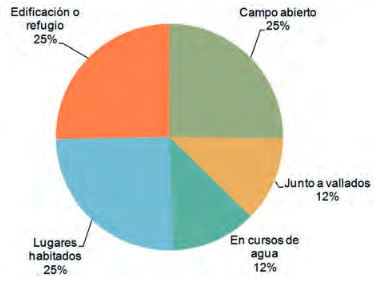
\includegraphics[width=0.4\textwidth]{4a6}
\caption{"Probabilidad de localización niños entre 4 a 6 Años"}
\end{figure}
\end{center}

\subsection{ULC y radio de busqueda}
El primer acecamiento que se real
\end{document}